\section{Implementazione}
\definecolor{codegreen}{rgb}{0,0.6,0}
\definecolor{codegray}{rgb}{0.5,0.5,0.5}
\definecolor{codepurple}{rgb}{0.58,0,0.82}
\definecolor{backcolour}{rgb}{0.95,0.95,0.92}

\hspace{\parindent}In questa sezione verranno illustrate le tecnologie utilizzate per la realizzazione dell'elaborato e verranno commentati dei tratti di codice fondamentali
\subsection{NDEF e Sicurezza}
\hspace{\parindent}NDEF è un preciso standard per un formato di dati sui chip NFC, viene utilizzato in applicazioni quali le carde di credito, o gli smart poster, la struttura di un messaggio è quella vista nella seguente figura: 
\begin{figure}[h]
\begin{center}
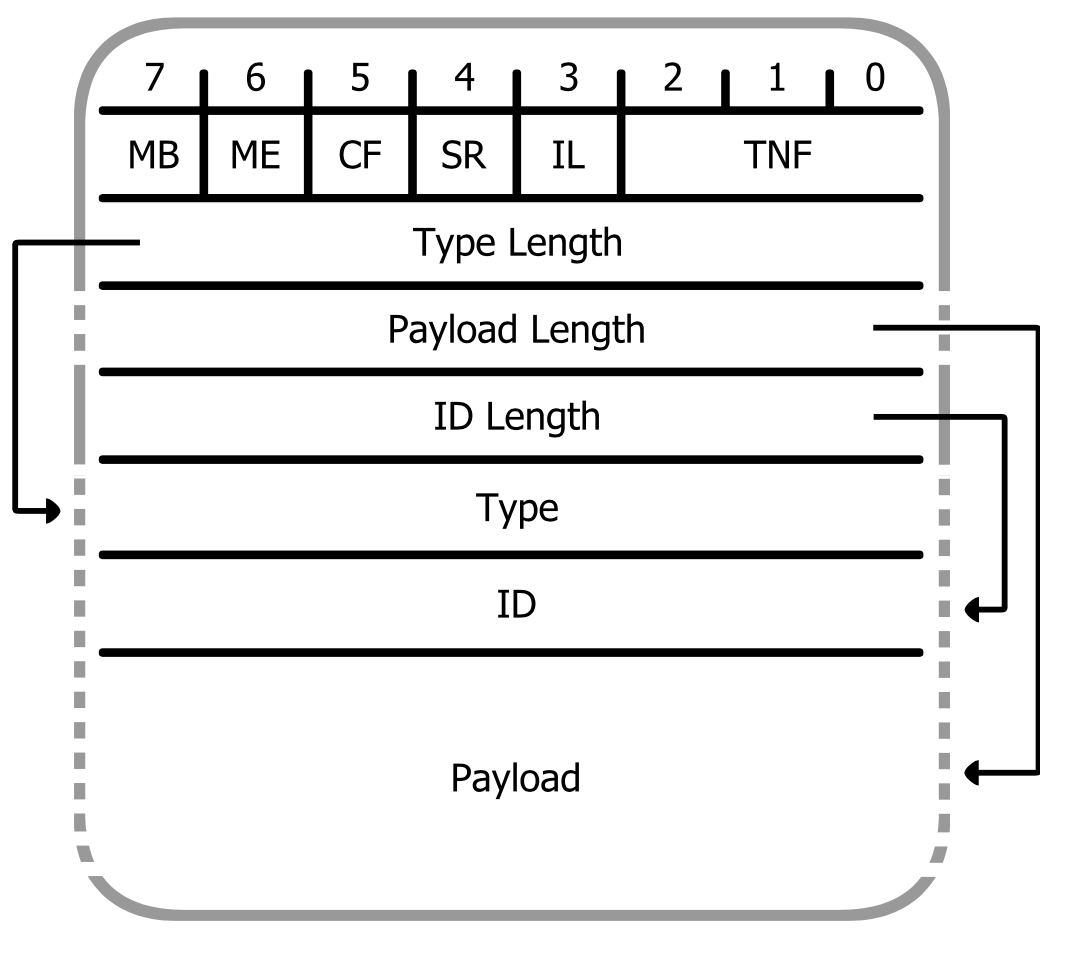
\includegraphics[scale=0.45]{ndefstructure}
\caption[NDEF Vulnerabilità]{Vulnerabilità NDEF\footnotemark}
\end{center}
\end{figure}
\footnotetext{\url{www.researchgate.net/publication/224227216_Security_Vulnerabilities_of_the_NDEF_Signature_Record_Type}}
In ordine abbiamo: 
\paragraph{Header}
Che è composto da: Message Begin (MB), Message End (ME), Chunk Flag (CF), Short record (SR), ID Length present (IL), Type Name Format (TNF), Length fields, Type, ID
\\I primi 5 parametri sono dei flag, per finire invece abbiamo il \textbf{Payload} che è il messaggio.
\\Detto questo andiamo a concentrarci meglio su determinati campi quindi:
\paragraph{•}CF: indica il record che fa parte di una catena di record, quando il suo valore è pari a 1 vuol dire che c'è \textit{almeno} 1 altro record nella catena, invece quando non è settato vuol dire che ci troviamo o nel caso di record singolo o nel caso di ultimo elemento della catena. Una cosa da notare è che ME e CF non possono essere entrambi settati a 1
\paragraph{•}SR: quando viene messo ad 1 vuol dire che il record corrente è di tipologia short, questo comporta che il campo Payload Length, che si trova dentro Length fields, viene espresso tramite 1 byte, in alternativa viene espresso da 4 byte
\paragraph{•} IL: indica se nel record è presente un identificatore, se non dovesse essere abilitato questo comporta che non vi saranno il campo ID Length e il campo ID che è quello di identificazione del record.
\paragraph{•}TNF: serve per indicare la struttura del campo Type, è composto da 3 bit e può assumere solo i valori da 0 a 6 perché il numero 7 è riservato.
\\\\NDEF ha anche una firma
\begin{figure}[h]
\begin{center}
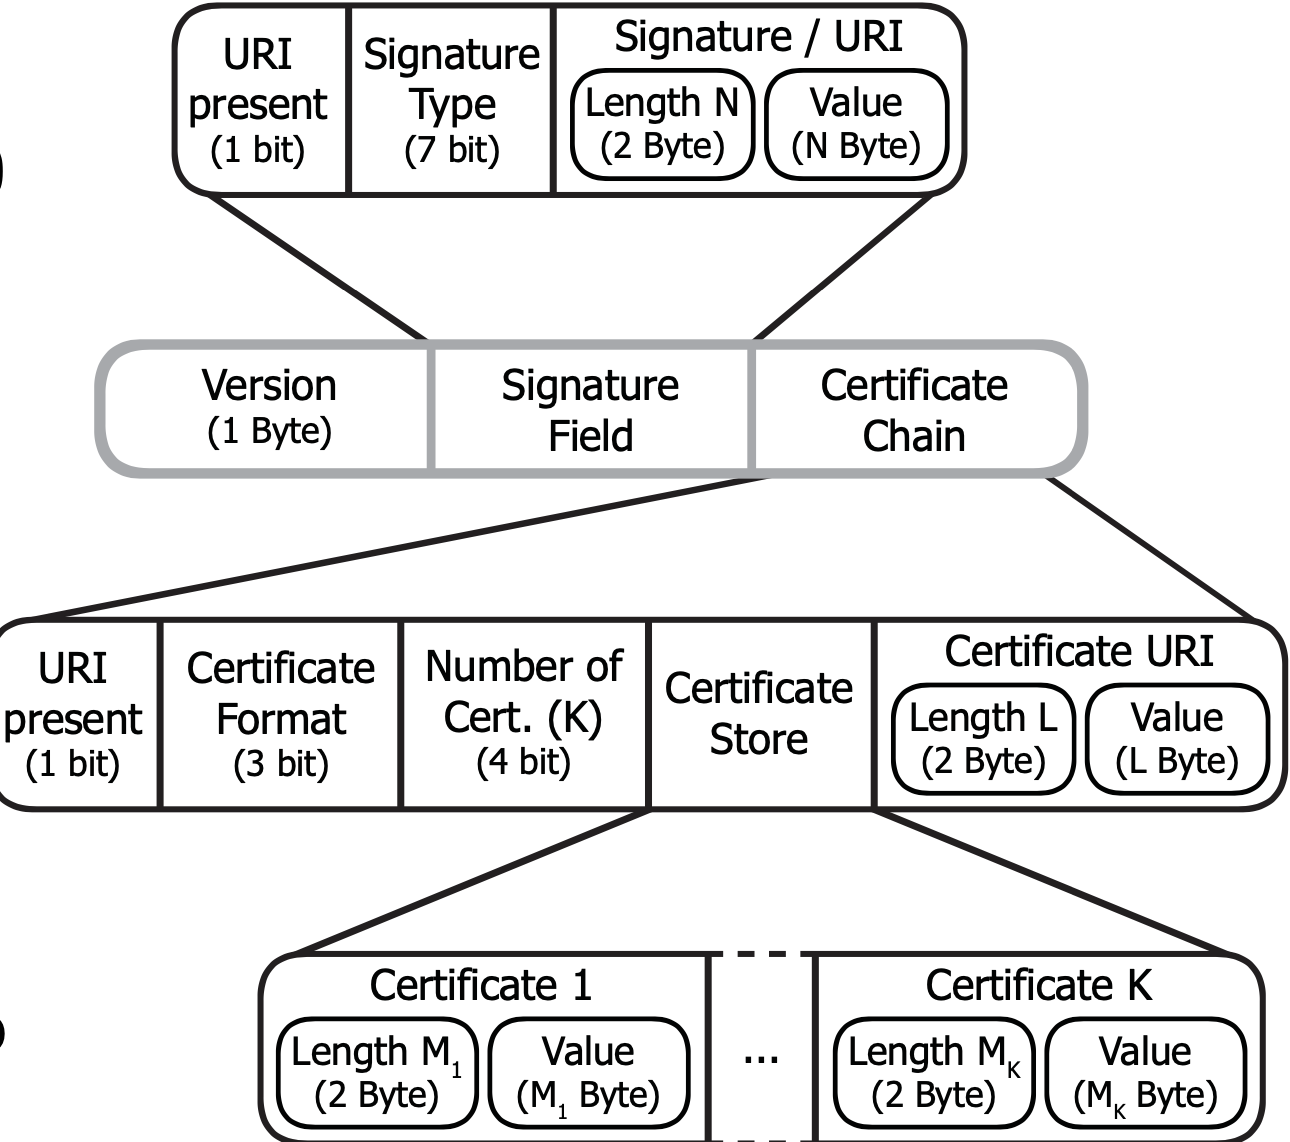
\includegraphics[scale=0.6]{ndefsign}
\caption[NDEF Vulnerabilità]{Vulnerabilità NDEF\footnotemark}
\end{center}
\end{figure}
\footnotetext{\url{www.researchgate.net/publication/224227216_Security_Vulnerabilities_of_the_NDEF_Signature_Record_Type}}
\\L'ultimo documento di specifica è stato rilasciato nel Novembre 2010, sostanzialmente ha una struttura fatta da un \textbf{campo firma}, che può essere una firma o una referenza URI ad una firma e da una \textbf{catena di certificati}, che è una catena di certificati PKI su un percorso sicuro.
\\Il record con la firma viene aggiunto ad una sequenza di record, e questo firma ogni record tra il record di firma appena precedente e se stesso, infatti un messaggio NDEF può contenere più di una firma.
\subsubsection{Cosa viene firmato?}
\hspace{\parindent} I campi che non vengono firmati sono MB/ME, questo perché se venissero firmati la firma non potrebbe essere agganciata al messaggio NDEF già firmato. Type, ID e Payload invece vanno firmati per assicurare l'integrità dei dati, mentre quando TNF viene cambiato, l'intero significato del record cambia, può essere quindi usato per nascondere dei record (identificati da type "Unknown"). 
\subsubsection{Sicurezza}
\hspace{\parindent}La tecnologia NFC è un'evoluzione dell'RFID, da un lato risulta meno predisposta ad attacchi esterni ma dall'altro lato è soggetta alle problematiche di sicurezza del suo predecessore. Le possibili minacce di sicurezza a cui sono sottoposti sono quelle riguardanti l'acquisizione, o l'alterazione dei dati contenuti nel tag, queste minacce possono avvenire mediante interrogazioni fraudolente o mediante l'intercettazione delle informazioni mediante ricevitori radio durante la lettura da parte di un lettore autorizzato.
\subsubsection{Intercettazioni}
\hspace{\parindent}Nell'ambito dell'NFC ma soprattutto in maniera generale, nel campo delle comunicazioni wireless l'intercettazione dei dati è uno degli attacchi più comuni. Per effettuare quest'attacco serve attrezzatura progettata ad hoc, quindi antenne e lettori fatti su misura. Per quanto riguarda il caso specifico NFC è un attacco molto difficile da realizzare a causa sei seguenti fattori:
\paragraph{i} potenza emessa dallo strumento sotto intercettazione
\paragraph{ii} fattori ambientali
\paragraph{iii} presenza della crittografia

Quindi da questo capiamo che anche in base al tipo di tag \footnote{cap 2 par 2.3.1} un attacco può essere più facile o più difficile, per esempio un attacco su un tag di tipo 1 sarà molto più semplice che su un tag di tipo 4.
\\Ci sono anche contromisure come per esempio quella di diminuire il campo magnetico, magari aumentando il fattore di direzionalità delle antenne, oppure usare algoritmi di cifratura per il messaggio, algoritmi per esempio AES.
\subsubsection{Modifica dei dati}
\hspace{\parindent}La modifica dei dati è un problema molto pericoloso, questo perché risulta trasparente all'utente, ha come scopo quello di modificare i dati trasmessi e renderli "validi". Fortunatamente risulta un attacco molto difficile da eseguire perché bisognerebbe riuscire ad intercettare completamente ogni bit del messaggio e rimandarlo sulle frequenze precise, quindi ogni volta modulando il campo delle frequenze in modo specifico e diverso.
\subsubsection{Man in the middle}
\hspace{\parindent}È uno degli attacchi più pericolosi, infatti può arrecare molti danni ai sistemi coinvolti. Mentre sysA e sysB stanno comunicando, sysH, il dispisitivo dell'hacker, si interpone tra di loro. Durante la comunicazione sysH altera il dialogo che hanno sysA e sysB, mettendosi in mezzo e fingendosi sysA per sysB e sysB per sysA. La soluzione a questo attacco è quella di instaurare un canale sicuro, quindi usando una chiave per criptare i dati. 
Potrebbe succede che sysH cerchi di negoziare una chiave ai due sistemi però è molto complesso perché richiederebbe la visibilità di sysH.

\subsection{UUID}
\hspace{\parindent}Un UUID\footnote{https://tools.ietf.org/html/rfc4122} conosciuto anche come Universally Unique Identifier, è un numero di 128 bit utilizzato per identificare informazioni nei sistemi informatici, lo si può trovare nell'rfc 4122.
\subsubsection{Come è formato?}
\hspace{\parindent}Il codice è composto da 16 byte, solitamente viene identificato da 32 caratteri esadecimali, a livello di sicurezza assume $ 3 \cdot 10^{38}$ possibili combinazioni
\begin{center}
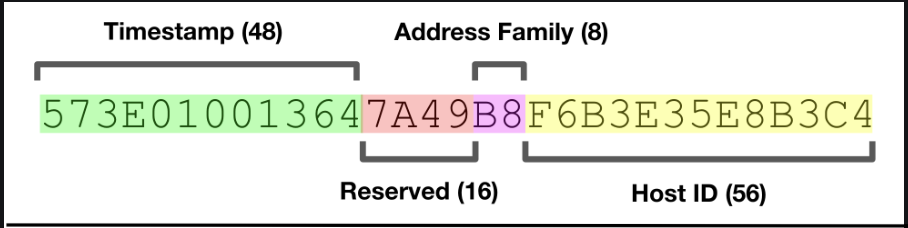
\includegraphics[scale=0.5]{uuid}
\end{center}
A differenza di altri sistemi l'unicità del codice generato non dipende da un'autorità centrale di registrazione o dal coordinamento delle parti che lo generano, però la sua probabilità di essere duplicato è talmente vicina a zero che viene considerata trascurabile.

\subsubsection{Analisi a livello matematico}

\hspace{\parindent}Considerando i 128 bit dell'UUID versione 4, 6 bit vengono riservati, quattro per la versione e due per altri parametri, quindi un UUID generato randomicamente ha 122 bit casuali. La probabilità che due UUID hanno lo stesso valore può essere calcolata usando la teoria delle probabilità (Paradosso del compleanno \footnote{https://betterexplained.com/articles/understanding-the-birthday-paradox/}). Usando quindi quest'approssimazione possiamo calcolare:
\begin{equation}
p(n) \approx 1- e^{-\frac{n^2}{2\cdot 2^x}}
\end{equation}
Notiamo quindi che quando il termine $ \frac{n^2}{2\cdot 2^x}$ è vicino allo zero, la probabilità può essere direttamente approssimata in questo modo:
\begin{equation}
p(n) \approx \frac{n^2}{2\cdot 2^x}
\end{equation}
Analizzandolo quindi in modo numerico potremo pensare che anche generando 1 miliardo di UUID ogni secondo per i prossimi 100 anni la probabilità di creare almeno un duplicato sarebbe circa del 50\%.


\subsection{Analisi del codice}
\hspace{\parindent}In questa sezione verranno mostrati i frammenti più importanti del codice
\lstdefinestyle{mystyle}{
    backgroundcolor=\color{backcolour},   
    commentstyle=\color{codegreen},
    keywordstyle=\color{magenta},
    numberstyle=\tiny\color{codegray},
    stringstyle=\color{codepurple},
    basicstyle=\ttfamily\footnotesize,
    breakatwhitespace=false,         
    breaklines=true,                 
    captionpos=b,                    
    keepspaces=true,                 
    numbers=left,                    
    numbersep=5pt,                  
    showspaces=false,                
    showstringspaces=false,
    showtabs=false,                  
    tabsize=2
}
\lstset{style=mystyle}
\subsubsection{Avvio del Database NoSQL}
\lstinputlisting[language=bash]{./Code/avvio.sh}

Automaticamente il controllore mettendo i suoi dati (validi) apre la connessione al database e va direttamente alla pagina di controllo degli abbonamenti.
\subsubsection{Creazione del Database}
\lstinputlisting[language=bash]{./Code/CreazioneDB.sh}

La creazione del database viene fatta una sola volta, prima del rilascio dell'applicazione. 
\\Potrebbero succedere problemi hardware, oppure il link potrebbe perdere la connessione magari durante un processamento dei dati, per questo una soluzione è quella di avere un backup disponibile appena succede un problema, quindi i dati vengono replicati per assicurare che non ci siano fallimenti. Cassandra posiziona le repliche dei dati su nodi diversi in base a due fattori:
\paragraph{•} Strategia di replicazione
\paragraph{•} Fattore di replicazione
Il primo dice dove posizionare le replica, il secondo invece determina quante repliche vengono posizionate, un esempio lo troviamo nella riga 4 dove abbiamo la stringa \textit{'replication\_factor' : 3}, questo indica che vengono fatte 3 repliche su 3 nodi diversi. Solitamente per garantire che non ci siano fallimenti il fattore di replicazione deve essere 3.
\\Nella riga 3 vediamo la stringa \textit{'SimplyStrategy'}, questa viene usata quando abbiamo un solo data center, quindi la prima replica viene posizionata sul nodo selezionato dal partizionatore, dopo questo, le restanti repliche vengono posizionate in senso orario a partire dalla direzione del nodo.
\subsubsection{Creazione tabella nel Database}
\lstinputlisting[language=bash]{./Code/CreazioneTabella.sh}

Anche questa parte di codice, come la creazione del database viene fatta una sola volta, prima del lancio dell'applicazione
\subsubsection{Connnessione al database mediante CQLSH}
\lstinputlisting[language=bash]{./Code/ConnessioneCQLSH.sh}

In questo frammento viene mostrata la connessione con CQLSH ed un esempio di query. Nella riga 3 e 4 vediamo la risposta che viene data in output non appena effettuiamo la connessione, per effettuare la connessione è obbligatorio aver attivato il database\footnote{cap 3.3.1 }, altrimenti il servizio non sarà attivo e quindi ci sarà un errore nella connessione di tipo \textit{Connection Refused}.
\bigskip\subsubsection{Connessione al Database NoSQL}
\lstinputlisting[language=Java]{./Code/Connessione.java}

In questo frammento di codice viene mostrato il metodo con il quale viene fatta la connessione al database NoSQL Cassandra!
\subsubsection{Apertura della connessione con la porta seriale in Java}
\lstinputlisting[language=Java]{./Code/AperturaSeriale.java}

Nel frammento di codice appena visto c'è la dichiarazione delle porte che si vanno ad utilizzare, il \textbf{DATA\_RATE}, ovvero la quantità di dati digitali che possono essere trasferiti su un canale in un determinato intervallo temporale e l'apertura della connessione tramite la funzione \textbf{portId.open}.
\subsubsection{Rilevamento presenza tag NFC Arduino}
\lstinputlisting[language=c++]{./Code/RilevamentoPresenze.cpp}

In questo frammento di codice viene evidenziato come il chip NFC se presente viene scannerizzato, l'unica cosa che verrà presa sarà il payload e non l'intestazione! Questo perché l'intestazione ci serve solo a sapere se il chip è formattato in formato NDEF.
\subsubsection{Creazione abbonamento in Java}
\lstinputlisting[language=Java]{./Code/CreazioneAbbonamento.java}

Nella prima riga notiamo subito la variabile \textit{zoneatt}, in questa vi saranno le zone selezionate in precedenza per la creazione dell'abbonamento, nella riga numero 6 notiamo il comando importantissimo \textit{output.write(zoneatt)}, questo comando ci permette di scrivere sulla porta seriale le zone, che verranno successivamente codificate e poi scritte sul tag NFC.
\subsubsection{Scrittura abbonamento nel Database}
\lstinputlisting[language=Java]{./Code/ScritturaDB.java}

Le righe 5 e 6 servono per definire i parametri per la connessione, quindi indirizzo IP e porta, la linea 3 serve ad istanziare l'oggetto client che sarà quello che ci permetterà la connessione al database e la linea 9 ci permetterà l'apertura della connessione col database.
\\Andando avanti nel codice creiamo un abbonamento nel quale vengono passati i parametri da specifiche funzioni\footnote{I parametri sono presi dalla form di creazione dell'abbonamento e vengono crittografati}, per finire troviamo il comando più importante \textit{client.esegui()}, questo ci permetterà l'inserimento dei dati nel database, infatti eseguirà questo comando:
\begin{center}
\lstinputlisting[language=sql]{./Code/Query.sql.txt}
\end{center}
\subsubsection{Scrittura abbonamento su tag NFC }
\lstinputlisting[language=c++]{./Code/scritturaAbbonamento.cpp}

In questo frammento si mostra la scrittura del messaggio sul chip NFC, importante è l'istruzione alla linea 3, dove definiamo l'oggetto \textit{NdefMessage}, che sarà esattamente il tipo del tag, la funzione invece per scrivere direttamente sul chip è alla linea 6, ed è \textit{nfc.write(message)}, dopo di questa vengono fatti controlli per verificare che effettivamente il tag sia stato scritto.
\subsubsection{Lettura dell'abbonamento Java}
\lstinputlisting[language=java]{./Code/lettura.java}

Una delle istruzioni più importanti la troviamo nella prima linea, questa si attiva ogni volta che sulla porta seriale ci sono dei dati disponibili! Andando avanti nel codice notiamo che vengono fatti vari cicli, questi servono per identificare le zone e per vedere se effettivamente è un abbonamento di MyNBS o no.